
\chapter{Overall Description} \label{chp:overall-description}

\section{Product Perspective}
	\begin{comment}
		$<$Describe the context and origin of the product being specified in this SRS.  
		For example, state whether this product is a follow-on member of a product 
		family, a replacement for certain existing systems, or a new, self-contained 
		product. If the SRS defines a component of a larger system, relate the 
		requirements of the larger system to the functionality of this software and 
		identify interfaces between the two. A simple diagram that shows the major 
		components of the overall system, subsystem interconnections, and external 
		interfaces can be helpful.$>$
	\end{comment}
	The idea of good computational library should provided two crucial aspects. It should deliver correct (expected) result, highly performed (written in very optimal way) and additionally convenient in use. It is also very important to provide maximum of interoperability for the user to give the most flexible solution in terms of software applications.
	\begin{wrapfigure}{r}{0.5\textwidth} 
		\centering
		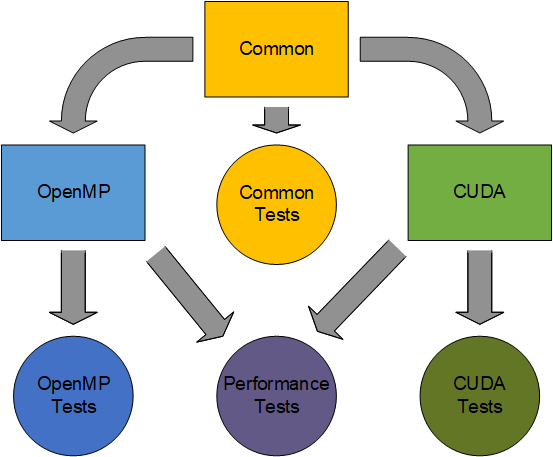
\includegraphics[scale=0.5]{img/overall-diagram}
		\caption{Block diagram of simulator.}
		\label{fig:block-diagram-of-library}
	\end{wrapfigure}

	Computation library was divided into three main components shown in Figure \ref{fig:block-diagram-of-library}. First component -- \emph{Common} will contain set of routines to transform \gls{MM} format to \gls{CRS} and \gls{ELL}. This part of software also contains classes that provides routines for solving matrix--vector product in serial. \emph{\gls{openmp}} contains solution that solves routine for matrix--vector product written using multiple threads. Third components solves the problem with help of NVIDIA Graphics card using \emph{\gls{cuda}} Toolkit Framework. 
	
	All main components contains corresponding test projects that checks for correctness of solving routines and sub-routines used in order to provide the matrix--vector product solution. This approach allows to maintain computational library in very convenient way without exposing existing software to bugs while adding or refactoring routines. Last component -- \emph{Performance Tests} checks the performance of created solutions on the set of arbitrarily chosen sparse matrices.
\section{Product Functions}
	\begin{comment}
		$<$Summarize the major functions the product must perform or must let the user 
		perform. Details will be provided in Section 3, so only a high level summary 
		(such as a bullet list) is needed here. Organize the functions to make them 
		understandable to any reader of the SRS. A picture of the major groups of 
		related requirements and how they relate, such as a top level data flow diagram 
		or object class diagram, is often effective.$>$
	\end{comment}
	
	The main function of a computational library briefly described in Chapter \ref{chp:overall-description} is to provided a functionality to calculate matrix--vector product for sparse matrices in \gls{CRS} and \gls{ELL} formats using parallel frameworks such as \gls{openmp} and \gls{cuda}.
\section{User Classes and Characteristics}
	\begin{comment}
		$<$Identify the various user classes that you anticipate will use this product.  
		User classes may be differentiated based on frequency of use, subset of product 
		functions used, technical expertise, security or privilege levels, educational 
		level, or experience. Describe the pertinent characteristics of each user class.  
		Certain requirements may pertain only to certain user classes. Distinguish the 
		most important user classes for this product from those who are less important 
		to satisfy.$>$
	\end{comment}
	User of this product is not highly specified although it is allowed to assume that most of the users will have a computer science background with focus on computational methods and techniques. 
\section{Operating Environment}
	\begin{comment}
		$<$Describe the environment in which the software will operate, including the 
		hardware platform, operating system and versions, and any other software 
		components or applications with which it must peacefully coexist.$>$
	\end{comment}
	\basicreq{OE}{System Specification}{Medium}
	{
		Library should be compatible with Linux and Windows environments. Also \gls{cuda} Toolkit Runtime Library should also be provided in order to run computations on graphics card.
	}\label{req:operating-enviornment:system-specification}
	\basicreq{OE}{Hardware Specification}{Low}
	{
		Library does not require any additional hardware requirements although in order to use \gls{cuda} routines it is necessary to have NVIDIA graphics card.
	}\label{req:operating-enviornment:hardware-specification}
\section{Design and Implementation Constraints}
	\begin{comment}
		$<$Describe any items or issues that will limit the options available to the 
		developers. These might include: corporate or regulatory policies; hardware 
		limitations (timing requirements, memory requirements); interfaces to other 
		applications; specific technologies, tools, and databases to be used; parallel 
		operations; language requirements; communications protocols; security 
		considerations; design conventions or programming standards (for example, if the 
		customer’s organization will be responsible for maintaining the delivered 
		software).$>$
	\end{comment}
	\basicreq{CNST}{Portability}{Medium}
	{ 
		Library should be portable across all operating systems that support compilation of \emph{C++} code.
	}
	\basicreq{CNST}{\glsdesc{MM} supported formats}{Medium}
	{ 
		Library should support transformation from general and symmetric formats that have pattern or real values presented in coordinates scheme.
	}
\section{User Documentation}
	\begin{comment}
		$<$List the user documentation components (such as user manuals, on-line help, 
		and tutorials) that will be delivered along with the software. Identify any 
		known user documentation delivery formats or standards.$>$
	\end{comment}
	\basicreq{USR-DOC}{Format of documentation}{Medium}
	{
		All the necessary information about usage of library should be available from the comments in header files.   
	}
\section{Assumptions and Dependencies}
	\begin{comment}
		$<$List any assumed factors (as opposed to known facts) that could affect the 
		requirements stated in the SRS. These could include third-party or commercial 
		components that you plan to use, issues around the development or operating 
		environment, or constraints. The project could be affected if these assumptions 
		are incorrect, are not shared, or change. Also identify any dependencies the 
		project has on external factors, such as software components that you intend to 
		reuse from another project, unless they are already documented elsewhere (for 
		example, in the vision and scope document or the project plan).$>$
	\end{comment}
	\basicreq{ASM-DEP}{Obligatory resources}{Very High}
	{
		Library should not use any external libraries. Although \gls{cuda} Toolkit Runtime library should be provided.
	}